\documentclass{article}
\usepackage{graphicx}
\usepackage{hyperref}
\usepackage{geometry}
\usepackage{xcolor}
\usepackage{tcolorbox}
\usepackage{tikz}
\usetikzlibrary{positioning, shapes.geometric, arrows.meta, shadows, backgrounds, calc}
\usepackage{fancyhdr}
\pagestyle{fancy}
\usepackage{pgf-pie} 
\usepackage[utf8]{inputenc}
\usepackage{enumitem}
\usepackage{amsmath}
\usepackage{titlesec}
\usepackage{multicol}
\hypersetup{
  colorlinks=true,
  linkcolor=black,
  urlcolor=blue,
  citecolor=black,
  pdfborder={0 0 0}
}

% Page margins
\geometry{margin=1in}

% Define your palette colors
\definecolor{headerColor}{HTML}{D2B48C} % Tan
\definecolor{primaryColor}{HTML}{8B5A2B} % Brownish
\definecolor{backgroundColor}{HTML}{F4E4C1} % Light beige
\definecolor{sectionColor}{HTML}{F9F9F9} % Very light gray
\definecolor{accentColor}{HTML}{FF6F61} % Vibrant coral

\hypersetup{
  colorlinks=true,
  linkcolor=primaryColor, % <-- Make sure this line is there
  urlcolor=blue,
  citecolor=black,
  pdfborder={0 0 0}
}
% Custom title page with background
\newenvironment{CustomTitlePage}{
  \begin{titlepage}
  \begin{tikzpicture}[remember picture, overlay]
    \shade[left color=orange!20, right color=orange!10]
      (current page.south west) rectangle (current page.north east);
  \end{tikzpicture}
  \vspace*{2cm}
}{
  \end{titlepage}
}

\begin{document}
% ALL content for the first page inside this environment
\begin{CustomTitlePage}
\centering
    % Main Title
    {\Huge \bfseries \color{primaryColor} RebelInuX White Paper} \\[0.5em]
    % Coin's name
    {\large \textit{RebelInuX (REBL)}} \\[0.5em]
    % Author
    {\large \textit{Clément Landormy, Founder of RebelInuX}} \\[0.5em]
    % Date
    {\large \today} \\[2em]
    % Optional: Add a small logo or icon if you like
    % \includegraphics[width=0.2\textwidth]{your-logo.png} \\[2em]
    % Subtle separator line
    \rule{\textwidth}{0.4pt} \\[2em]
    % Main header or subtitle
    {\LARGE \color{black} The Rebellious Meme Coin Backed by a Pack of NFT Rebels!} \\[3em]
    % Image
    \includegraphics[width=0.4\textwidth]{RebelInuX.jpg} \\[2em]
    % Intro box
\begin{tcolorbox}[colback=headerColor!15, colframe=headerColor, boxrule=1.5pt, width=0.75\textwidth, arc=4mm]
    \centering
    {\Large \bfseries Introduction} \\[0.5em]
    \textbf{RebelInuX} pioneers a novel meme coin model with a \textbf{triple-asset ecosystem} on ZORA. This creates a direct link between \textbf{digital ownership} of a Creator Coin, \textbf{community identity} with a Content Coin NFT, and \textbf{\$REBL token rewards}, merging collectible art with a secure claim mechanism.\\

    Inspired by the \textbf{fearless Shiba Inu} spirit, we embody \textbf{rebellion}, \textbf{humor}, and \textbf{decentralization}. Our ultimate goal is to achieve complete decentralization, transferring all control to the community and eliminating any central points of failure. By acquiring the core duo of assets, holders become \textbf{core participants} in our community and gain the ability to claim \textbf{\$REBL tokens} across chains. Join us as we disrupt and redefine the meme coin landscape.
\end{tcolorbox}
\end{CustomTitlePage}

\fancyhf{}
\fancyhead[C]{RebelInuX \textbar\  Join us: \href{https://x.com/RebelInuX}{Twitter} | \href{https://t.me/+bNrP-ozjM501YWVk}{Telegram} | \href{https://discord.gg/3gBzGY6j}{Discord} | \href{https://zora.co/@rebelinuxZORA}{Zora}}
\fancyfoot[C]{\thepage}

% Rest of document starts here
\newpage
\tableofcontents
\newpage

\section[
  \texorpdfstring{\color{primaryColor}RebelInuX Architecture Overview}{RebelInuX Architecture Overview}
]{\color{primaryColor}\textbf{RebelInuX Architecture Overview}}
\label{sec:Architecture} 
\begin{center}
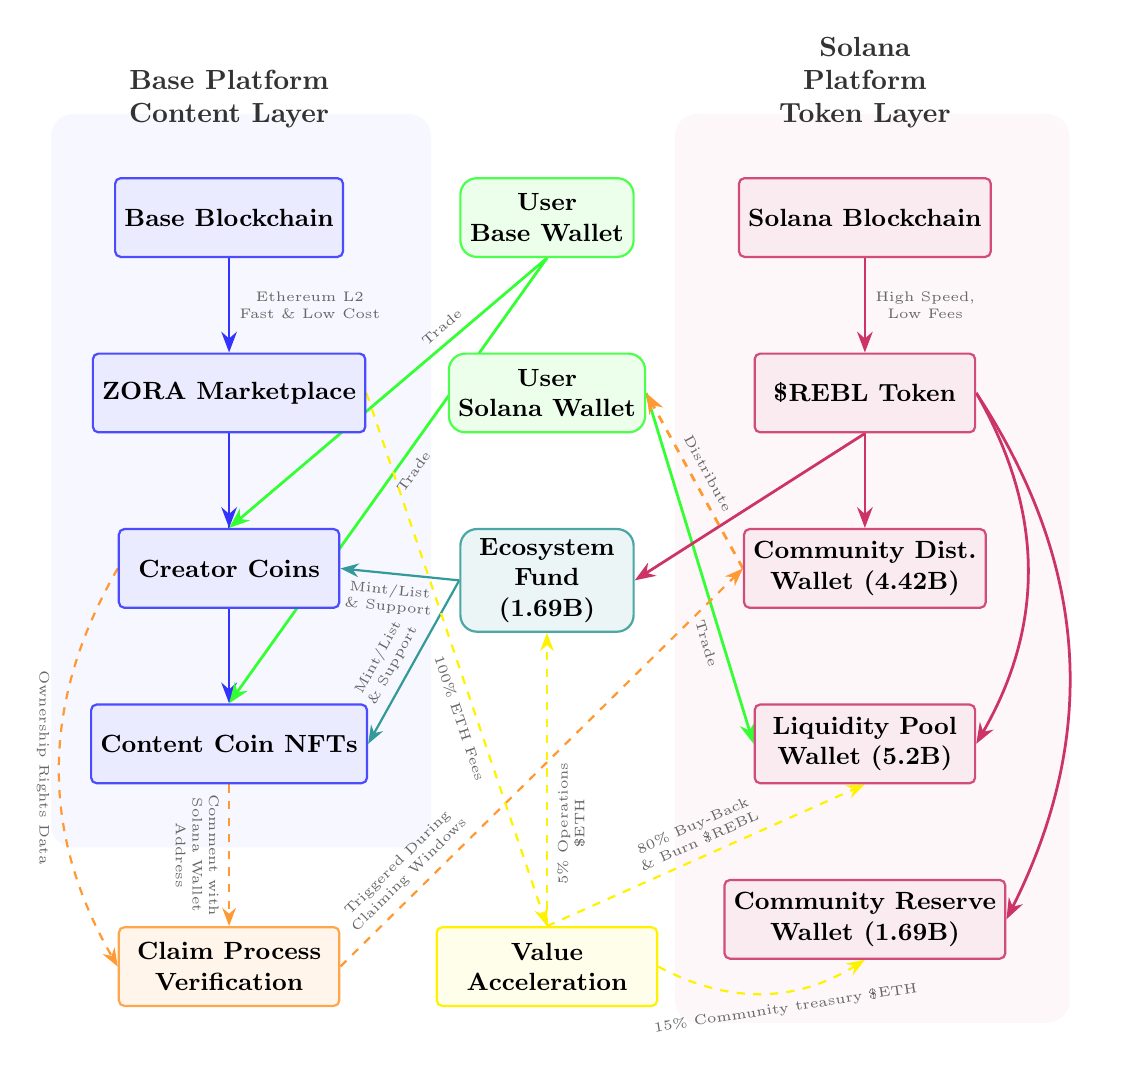
\begin{tikzpicture}[
    node distance=1.2cm and 0.8cm,
    baseNode/.style={rectangle, draw=blue!70, fill=blue!8, thick, minimum height=1cm, minimum width=2.8cm, align=center, font=\small\bfseries, rounded corners=2pt},
    solanaNode/.style={rectangle, draw=purple!70, fill=purple!8, thick, minimum height=1cm, minimum width=2.8cm, align=center, font=\small\bfseries, rounded corners=2pt},
    userNode/.style={rectangle, draw=green!70, fill=green!8, thick, rounded corners=6pt, minimum height=1cm, minimum width=2.2cm, align=center, font=\small\bfseries},
    creatorNode/.style={rectangle, draw=teal!70, fill=teal!8, thick, rounded corners=6pt, minimum height=1cm, minimum width=2.2cm, align=center, font=\small\bfseries},
    claimNode/.style={rectangle, draw=orange!70, fill=orange!8, thick, minimum height=1cm, minimum width=2.8cm, align=center, font=\small\bfseries, rounded corners=2pt},
        valueaccelerationNode/.style={rectangle, draw=yellow, fill=yellow!8, thick, minimum height=1cm, minimum width=2.8cm, align=center, font=\small\bfseries, rounded corners=2pt},
    arrow/.style={-Stealth, scale=1.0, thick, line width=1pt},
    label/.style={text width=2.8cm, align=center, font=\normalsize\bfseries, text=black!80},
    smallLabel/.style={font=\tiny, text=black!60}
]

% Nodes - DEFINE NODES FIRST
% Base Chain
\node[baseNode] (baseChain) {Base Blockchain};
\node[baseNode, below=of baseChain] (zora) {ZORA Marketplace};
\node[baseNode, below=of zora] (creatorCoin) {Creator Coins};
\node[baseNode, below=of creatorCoin] (contentNFT) {Content Coin NFTs};

% Solana Chain
\node[solanaNode, right=5cm of baseChain] (solanaChain) {Solana Blockchain};
\node[solanaNode, below=of solanaChain] (reblToken) {\$REBL Token};
\node[solanaNode, below=of reblToken] (communityWallet) {Community Dist.\\Wallet (4.42B)};
\node[solanaNode, below=of communityWallet] (liquidityPool) {Liquidity Pool\\Wallet (5.2B)};
\node[solanaNode, below=of liquidityPool] (communityReserve) {Community Reserve\\Wallet (1.69B)};


% Wallets - ALL IN SAME CENTER COLUMN
\node[userNode] at ($(baseChain)!0.5!(solanaChain)$) (userBase) {User\\Base Wallet};
\node[userNode, below=of userBase] (userSolana) {User\\Solana Wallet};
\node[creatorNode, below=1.2cm of userSolana] (creatorWallet) {Ecosystem\\ Fund \\ (1.69B)};

% Processes
\node[claimNode, below=1.8cm of contentNFT] (claimProcess) {Claim Process\\Verification};
\node[valueaccelerationNode, below=3.725cm of creatorWallet] (buyBack) {Value \\ Acceleration};

% Chain Labels
\node[label, above=0.5cm of baseChain] {Base Platform\\Content Layer};
\node[label, above=0.5cm of solanaChain] {Solana Platform\\Token Layer};

% Background fills - drawn first (lowest layer) - PLACE AFTER NODES ARE DEFINED
\begin{scope}[on background layer]
    \fill[blue!3, rounded corners=8pt] ([xshift=-0.8cm,yshift=0.8cm]baseChain.north west) rectangle ([xshift=0.8cm,yshift=-0.8cm]contentNFT.south east);
    \fill[purple!3, rounded corners=8pt] ([xshift=-0.8cm,yshift=0.8cm]solanaChain.north west) rectangle ([xshift=0.8cm,yshift=-0.8cm]communityReserve.south east);
\end{scope}

% Arrows - drawn in middle layer (above background, below nodes) - PLACE AFTER NODES
\begin{scope}[on background layer]
    % Base chain connections
    \draw[arrow, blue!80] (baseChain.south) to 
    node[right, smallLabel, align=center, pos=0.5] {Ethereum L2\\ Fast \& Low Cost}(zora.north);
    \draw[arrow, blue!80] (zora.south) -- (creatorCoin.north);
    \draw[arrow, blue!80] (zora.south) -- (contentNFT.north);
    % User connections
    \draw[arrow, green!80] (userBase.south) to node[above,sloped, smallLabel, pos=0.3] {Trade} (creatorCoin.north);
    \draw[arrow, green!80] (userBase.south) to node[below, sloped, smallLabel, pos=0.46] {Trade} (contentNFT.north);
    \draw[arrow, green!80] (userSolana.east) to node[below,sloped, smallLabel, pos=0.7] {Trade} (liquidityPool.west);

    % Creator connections
        \draw[arrow, teal!80, thick] (creatorWallet.west) to
        node[below, sloped, smallLabel, align=center , pos=0.57] {Mint/List \\\& Support} (creatorCoin.east);
                \draw[arrow, teal!80, thick] (creatorWallet.west) to
        node[above, sloped, smallLabel, align=center , pos=0.57] {Mint/List \\\& Support} (contentNFT.east);

    % Solana chain connections
        \draw[arrow, purple!80] (solanaChain.south) to 
    node[right, smallLabel, align=center, pos=0.5] {High Speed,\\Low Fees}(reblToken.north);
    \draw[arrow, purple!80] (reblToken.south) -- (communityWallet.north);
    \draw[arrow, purple!80] (reblToken.east) to [bend left=30](liquidityPool.east);
        \draw[arrow, purple!80] (reblToken.east) to [bend left=30](communityReserve.east);
    \draw[arrow, purple!80] (reblToken.south) to(creatorWallet.east);

    % Cross-chain connections
    \draw[arrow, dashed, orange!80, thick] (contentNFT.south) to
        node[below, sloped, smallLabel, align=center] {Comment with \\ Solana Wallet \\ Address} (claimProcess.north);
                    \draw[arrow, dashed, orange!80, thick] (creatorCoin.west) to[bend right=30]
        node[below, sloped, smallLabel, align=center] {Ownership Rights Data}(claimProcess.west);
    \draw[arrow, dashed, orange!80, thick] (claimProcess.east) to
        node[above, smallLabel,sloped, align=center, pos=0.20] {Triggered During \\ Claiming Windows} (communityWallet.west);
            \draw[arrow, dashed, orange!80] (communityWallet.west) to node[above,sloped, smallLabel, pos=0.5] {Distribute} (userSolana.east);

    % Value acceleration loop
    \draw[arrow,dashed, yellow, thick] (zora.east) to 
        node[below, sloped, smallLabel, align=center, pos=0.6] {100\% ETH Fees} (buyBack.north);
    \draw[arrow, dashed, yellow, thick] (buyBack.north) to
        node[above,sloped,smallLabel, align=center] {80\% Buy-Back \\\& Burn \$REBL} (liquidityPool.south);
    \draw[arrow, dashed, yellow, thick] (buyBack.east) to[bend right=30]
        node[below, sloped, smallLabel, align=center, pos=0.6] {15\% Community treasury \$ETH} (communityReserve.south); 
    \draw[arrow, dashed, yellow, thick] (buyBack.north) to 
        node[below, sloped, smallLabel, align=center, pos=0.35] {5\% Operations \\\$ETH}(creatorWallet.south);
\end{scope}


\end{tikzpicture}
\end{center}

\begin{center}
    {\LARGE \color{primaryColor}\textbf{Legend of Diagram Symbols and Colors}}
\end{center}
\begin{multicols}{2}
\begin{itemize}
    \item \textbf{\textcolor{blue}{Blue Boxes and Arrows}}: Base Assets and their Connection to ZORA on the Base Blockchain
    \item \textbf{\textcolor{purple}{Purple Boxes and Arrows}}: Solana blockchain assets and initial token distributions
    \item \textbf{\textcolor{green}{Green Boxes and Arrows}}: User interactions and wallets
\end{itemize}
\columnbreak
\begin{itemize}
    \item \textbf{\textcolor{teal}{Teal Boxes and Arrows}}: Ecosystem fund interactions and wallets
        \item \textbf{\textcolor{yellow}{Yellow Boxes and Dashed Arrows}}: Value Acceleration Mechanism
    \item \textbf{\textcolor{orange}{Orange Boxes and Dashed Arrows}}: Token claim process and distribution
\end{itemize}
\end{multicols}
\vspace{0.5cm}
This visual overview illustrates how the RebelInuX ecosystem operates across multiple blockchains, with ZORA managing the content and community layer, and Solana handling the token economy and value accrual mechanisms. The architecture enables seamless cross-chain interactions while leveraging each platform's strengths to directly reward creator participation and drive value back to the entire ecosystem.


\section[
  \texorpdfstring{\color{primaryColor}The Triple-Asset Ecosystem}{The Triple-Asset Ecosystem}
]{\color{primaryColor}\textbf{The Triple-Asset Ecosystem}}
\label{sec:Triple-Asset} 
\begin{tcolorbox}[colback=headerColor!10!white, colframe=headerColor, boxrule=2pt, width=\textwidth, arc=6mm, left=8mm, right=8mm, top=6mm, bottom=6mm]

\subsection[
  \texorpdfstring{\color{primaryColor}Overview and Utility}{Overview and Utility}
]{\color{primaryColor}Overview and Utility}
The RebelInuX ecosystem is powered by a novel triple-asset model on \textbf{ZORA}, designed to merge community engagement with secure, verifiable value distribution. As illustrated in the \hyperref[sec:Architecture]{\textbf{Architecture Overview}}, this system operates across chains and consists of three interconnected assets that work together to distribute the \textbf{RebelInuX (\$REBL)} meme coin on Solana: % <-- REFERENCE ADDED HERE

\begin{itemize}
    \item \textbf{The Creator Coin: Your Digital Claim Ticket.} This is the core value-bearing asset. Each Creator Coin grants you a fixed allocation of \$REBL tokens from the Solana community pool, distributed during designated claim periods. Its ownership is the primary data point verified by the \textbf{Claim Process} shown in the architecture.
    \item \textbf{The Content Coin NFT: Your Identity \& Secure Bridge.} This NFT serves as your unique identity within the Rebel Pack and is the secure communication channel for the cross-chain claiming process (see \textbf{Figure~\ref{fig:contentcoin}}). It does not hold the claimable value itself but is essential for initiating the transfer, as it contains the Solana wallet address required for distribution.
    \item \textbf{The \$REBL Token: Your Cross-Chain Reward.} This is the final reward token distributed on Solana to holders of both core assets during claim periods. Its value is directly accelerated by the ecosystem's activity through the \textbf{Value Acceleration Mechanism}.
\end{itemize}

This innovative separation ensures security—your claim power (Creator Coin) and your cross-chain destination (provided via the Content Coin) are never held in a single, vulnerable location. By acquiring both core assets, you secure your membership in an exclusive pack with a direct, verifiable stake in the growth of \$REBL.
\end{tcolorbox}
\begin{center}
  \includegraphics[width=0.4\textwidth]{RebelInuX — visuals.JPG} % <-- Replace with your actual filename
  \\ % Line break for the caption
\small\textit{Figure 1:``RebelInuX — The ZORA Prophecy'' – A Content Coin NFT serving as your identity and secure bridge within the ecosystem. Explore the collection on: \href{https://zora.co/@rebelinux}{ZORA}}
  \label{fig:contentcoin}
\end{center}

\begin{tcolorbox}[colback=headerColor!10!white, colframe=headerColor, boxrule=2pt, width=\textwidth, arc=6mm, left=8mm, right=8mm, top=6mm, bottom=6mm]
\subsection[
  \texorpdfstring{\color{primaryColor}How to Claim \$REBL Tokens}{How to Claim \$REBL Tokens}
]{\color{primaryColor}How to Claim \$REBL Tokens}

The process to claim your \$REBL tokens is a secure, multi-step operation tied to specific claim periods:

\begin{enumerate}
    \item \textbf{Acquire the Core Duo of Assets:}
    \begin{itemize}
        \item \textbf{Purchase a Creator Coin:} This is your claim ticket. On our ZORA collection page, click the \textbf{"Trade"} button to acquire it. Ownership grants you a fixed allocation of \$REBL tokens.
        \item \textbf{Purchase a Content Coin NFT:} This is your secure communication key. To acquire it, navigate to any individual NFT in the collection and click the \textbf{"Buy"} button.
    \end{itemize}
    Both assets are available in our collection on the ZORA marketplace: \href{https://zora.co/@rebelinux}{https://zora.co/@rebelinux}.

    \item \textbf{Wait for a Claim Period:} Token distributions occur during designated, pre-announced claim periods (e.g., quarterly). The timing will be clearly communicated on our official channels. You only need to hold both core assets at the time of the snapshot for each claim period.
    \item \textbf{Initiate the Cross-Chain Claim:} When a claim period is active:
    \begin{itemize}
        \item Navigate to the ZORA page for your specific \textbf{Content Coin NFT}.
        \item \textbf{Leave a public comment containing your Solana public address.}
    \end{itemize}

    \begin{tcolorbox}[colback=red!5!white, colframe=red!75!black, title=\textbf{SECURITY WARNING}, fonttitle=\bfseries]
    \textbf{ONLY share your public address (e.g., \texttt{ahWDSP4...3MUiI}).} \\\textbf{NEVER} share your private key, seed phrase, or sign a malicious transaction.
    \end{tcolorbox}

    \item \textbf{Receive Your \$REBL Tokens on Solana:} Our system will scan for verified claims made during the active period. Upon confirmation, the \textbf{full amount} of your allocated \$REBL tokens for that period will be sent directly to your provided Solana wallet address.
\end{enumerate}
\end{tcolorbox}

\begin{tcolorbox}[colback=headerColor!10!white, colframe=headerColor, boxrule=2pt, width=\textwidth, arc=6mm, left=8mm, right=8mm, top=6mm, bottom=6mm]
\subsection[
  \texorpdfstring{\color{primaryColor}Benefits of Holding the Core Duo}{Benefits of Holding the Core Duo}
]{\color{primaryColor}Benefits of Holding the Core Duo}
\begin{itemize}
    \item \textbf{Guaranteed \$REBL Allocation:} Ownership of the \textbf{Creator Coin} grants you a right to a fixed allocation of \$REBL tokens, distributed over the claim periods. The \textbf{Content Coin NFT} is your key to securely claiming them.
    \item \textbf{Immediate Access:} Claim and receive the full amount of your tokens instantly during each active claim period, with no locking or vesting required.
    \item \textbf{Future Governance Rights:} Holders of both core assets are expected to be granted additional voting power or unique roles within the future RebelInuX DAO, recognizing their foundational role in the ecosystem.
    \item \textbf{Exclusive Access:} This pack will get first access to future distributions, community events, and partner collaborations, solidifying your status as a core rebel.
\end{itemize}
\end{tcolorbox}

% --- NEW SUBSECTION ADDED HERE ---
\begin{tcolorbox}[colback=headerColor!10!white, colframe=headerColor, boxrule=2pt, width=\textwidth, arc=6mm, left=8mm, right=8mm, top=6mm, bottom=6mm]
\subsection[
  \texorpdfstring{\color{primaryColor}Free Market Dynamics \& Incentives}{Free Market Dynamics \& Incentives}
]{\color{primaryColor}Free Market Dynamics \& Incentives}

The RebelInuX ecosystem is designed around free market principles and powerful incentives rather than artificial restrictions.

\begin{itemize}
    \item \textbf{No Artificial Lock-ups:} There is no protocol-level mechanism that prevents a holder from selling their Creator Coin after claiming \$REBL tokens. This ensures immediate liquidity and true ownership for all participants.
    \item \textbf{Value Accrual is the Incentive:} The primary incentive to hold the Creator Coin is the continuous value accrual from the \textbf{cross-chain buy-back mechanism}. As trading activity on ZORA generates ETH revenue used to buy and burn \$REBL, the value of the remaining unclaimed tokens backing each Creator Coin increases.
    \item \textbf{Speculation \& Utility:} The market price of the Creator Coin will reflect both the present value of its remaining claimable \$REBL and the speculative future value of its utilities, such as:
    \begin{itemize}
        \item Future governance power in the RebelInuX DAO.
        \item Exclusive access to community events and drops.
        \item Status as a core, foundational member of the rebellion.
    \end{itemize}
\end{itemize}

This model creates a transparent and efficient market where the value of the Creator Coin is directly tied to the success and activity of the entire RebelInuX ecosystem.
\end{tcolorbox}


\section[
  \texorpdfstring{\color{primaryColor}Current Tokenomics}{Current Tokenomics}
]{\color{primaryColor}\textbf{Current Tokenomics}}
\begin{tcolorbox}[colback=headerColor!10!white, colframe=headerColor, boxrule=2pt, width=\textwidth, arc=6mm, left=8mm, right=8mm, top=6mm, bottom=6mm]
% Introduction sentence
\textbf{The RebelInuX tokenomics are designed to promote sustainability, community growth, and project development through a transparent and fixed token allocation.}

\subsection[
  \texorpdfstring{\color{primaryColor}Emission Schedule}{Emission Schedule}
]{\color{primaryColor}Emission Schedule}

The total supply of RebelInuX tokens is fixed at \textbf{13 billion (13,000,000,000)} with \textbf{9 decimals}. No inflation or additional minting is planned; any future adjustments will be transparently communicated and community-governed.

\subsection[
  \texorpdfstring{\color{primaryColor}Token Distribution}{Token Distribution}
]{\color{primaryColor}Token Distribution}

\begin{itemize}
    \item \textbf{Ecosystem Fund (13\%) — 1.69B REBL:} This treasury is designated for ongoing development, protocol audits, marketing initiatives, and essential operational costs. To ensure long-term alignment and build trust, the entire allocation is subject to a transparent vesting schedule with an initial cliff, locking the majority of tokens for 2 years. \textbf{(See Subsection~\ref{subsec:Ecosystem} for details.)}
  \item \textbf{Community Reserve (13\%) — 1.69B REBL:}
    Strategic reserves locked until March 31, 2026. Upon unlock, full control will be transferred to the RebelInuX DAO for community-governed initiatives.
\textbf{(See Subsection~\ref{subsec:reserve} for details.)}
  \item \textbf{Liquidity Pool (40\%) — 5.2B REBL:}
    Funds liquidity on Raydium. The initial pool will consist of ~3.75B REBL. 90\% of its LP tokens are locked for 1 year; the remainder is reserved for future community-governed initiatives. \textbf{(See Section~\ref{sec:decentralization}.)}
  \item \textbf{Community Distribution (34\%) — 4.42B REBL:}
    Dedicated to rewarding holders of the RebelInuX Creator Coin and Content Coins. Tokens will be distributed according to the claim process outlined in \textbf{Section~\ref{sec:Triple-Asset}}.
\end{itemize}

\begin{center}
\begin{tikzpicture}
  % Draw the pie chart
  \node (chart) {
    \begin{tikzpicture}
      \pie[
        radius=3,
        color={orange!70, blue!70, green!70, gray!70},
        explode=0.05,
        text=legend,
      ]{
        13/Ecosystem Fund,
        13/Community Reserve,
        40/Liquidity Pool,
        34/Community Distribution
      }
    \end{tikzpicture}
  };

  % Add the title below the pie chart
  \node[below=0.5cm of chart] {\textit{\underline{Distribution of Tokens}}};
\end{tikzpicture}
\end{center}

\end{tcolorbox}



\begin{tcolorbox}[colback=headerColor!10!white, colframe=headerColor, boxrule=2pt, width=\textwidth, arc=6mm, left=8mm, right=8mm, top=6mm, bottom=6mm]
\subsection[
  \texorpdfstring{\color{primaryColor}Ecosystem Fund Vesting Schedule \& Security}{Ecosystem Fund Vesting Schedule \& Security}
]{\color{primaryColor}Ecosystem Fund Vesting Schedule \& Security}
\label{subsec:Ecosystem} 
The Ecosystem Fund is subject to the following vesting schedule, executed and enforced on-chain to guarantee long-term commitment and transparency:
\begin{itemize}
    \item \textbf{Platform:} StreamFlow.finance
    \item \textbf{Initial Cliff:} 20\% of allocation (2.6\% of total supply) unlocked at the start (TGE).
    \item \textbf{Linear Vesting:} The remaining 80\% of allocation vests linearly over a 24-month (2-year) period.
    \item \textbf{Current Governance:} The vested tokens are initially released to a secure multi-signature wallet controlled by the founder to prevent single-point-of-failure risks.
    \item \textbf{Future Governance:} The primary goal is to decentralize control. A community proposal will be initiated to transition the fund to a 3-of-5 multi-signature wallet governed by core contributors and established community members as the project grows.
\end{itemize}

\textbf{On-Chain Verification:}
\begin{itemize}
    \item \textbf{Ecosystem Fund Vesting Contract:} 
          \href{https://solscan.io/account/DVDBDPP6LpcBFRQWKDJU8L1QcQ7HXrVAg9j7dCJ7UqSv}{DVDBDPP6L...J7UqSv} (View on Solscan)
    
    \item \textbf{Initial Receiving Wallet (Multisig):} 
          \href{https://solscan.io/account/DGRMGRm6fWLs53ghWR7RFJ1JC8UvcKWQP9LtunQ1sa7R}{DGRMGRm6f...1sa7R} (View on Solscan)
\end{itemize}

\noindent\textit{Note: The vesting contract holds the tokens and controls their release schedule. The multisig wallet is the designated recipient of the unlocked tokens.}

\subsection[
  \texorpdfstring{\color{primaryColor}NFT Holder Reward Mechanism}{NFT Holder Reward Mechanism}
]{\color{primaryColor}NFT Holder Reward Mechanism}

The primary method for community distribution is through the \textbf{RebelInuX triple-asset ecosystem (Creator Coins, Content Coin NFTs, and \$REBL rewards) on ZORA}. The entire Community Distribution Wallet (4.42B \$REBL) on Solana is allocated to reward the holders of \textbf{Creator Coins}.

\subsection*{\color{primaryColor}Fixed Cross-Chain Allocation}

Each \textbf{Creator Coin} is linked to a fixed, predetermined amount of REBL tokens from the community pool on Solana. This creates a powerful cross-chain utility.

The total community distribution pool is 4.42 billion \$REBL. This entire amount will be distributed directly to Creator Coin holders. Therefore, the long-term value of each Creator Coin is pegged to this pool.

\textbf{Each RebelInuX Creator Coin represents a foundational claim of 4.42 \$REBL} on the Solana blockchain, drawn directly from the Community Distribution wallet. This fixed allocation will be distributed over specific claim periods.

Furthermore, the long-term utility of the Creator Coin is designed to evolve. A core proposition of the future RebelInuX DAO will be to discuss and vote on integrating the Community Reserve treasury into this claim mechanism. This would effectively grant each Creator Coin a potential future claim on a portion of the additional 1.69B \$REBL, significantly increasing its underlying value and solidifying its role as the ecosystem's primary value-accruing asset.


\subsection*{\color{primaryColor}Rationale}

This model directly aligns token distribution with proven community engagement (via ownership of the Creator Coin). It incentivizes long-term holding of the core asset and supports a healthy, stable market for \$REBL by distributing tokens through a controlled, claim-based process.

\end{tcolorbox}

\begin{tcolorbox}[colback=headerColor!10!white, colframe=headerColor, boxrule=2pt, width=\textwidth, arc=6mm, left=8mm, right=8mm, top=6mm, bottom=6mm]
\subsection[
  \texorpdfstring{\color{primaryColor}Community Reserve Wallet Utilization}{Community Reserve Wallet Utilization}
]{\color{primaryColor}Community Reserve Wallet Utilization}
\label{subsec:reserve}
The Community Reserve Wallet (1.69B \$REBL) is a treasury fund dedicated to the long-term health and growth of the RebelInuX ecosystem. \textbf{It is locked in a token lock  contract until March 31, 2026.}

% --- NEW ON-CHAIN VERIFICATION SUBSECTION ADDED HERE ---
\noindent\textbf{On-Chain Verification:}
\begin{itemize}
    \item \textbf{Token Lock Contract:} \href{https://solscan.io/account/GF3vv7NVEYGH4AmJexfzFKFerHRZ9mgmRiP1gA4Ap2Qt}{GF3vv7NV...A4Ap2Qt} (View on Solscan)
    \item \textbf{Designated Multisig Recipient:} \href{https://solscan.io/account/DGRMGRm6fWLs53ghWR7RFJ1JC8UvcKWQP9LtunQ1sa7R}{DGRMGRm6f...1sa7R} (View on Solscan)
\end{itemize}
% ------------------------------------------------------

Upon unlock, the full allocation will be securely transferred to the \textbf{RebelInuX Treasury Multisig wallet}. This serves as a secure, transitional holding vessel. The multisig's signers will then immediately facilitate the final, community-approved transfer of these funds to the dedicated treasury wallet of the RebelInuX DAO, completing the process of full decentralized community ownership.

\medskip % Adds a small vertical space for better readability

\noindent\textbf{Future Value Accrual to Creator Coins:} A primary goal for the DAO will be to propose and vote on mechanisms to integrate this community-owned treasury with the core triple-asset ecosystem. This could allow the RebelInuX Creator Coin to accrue value beyond its initial 4.42 \$REBL claim, potentially granting holders a right to a portion of the returns generated from this strategic community reserve, further solidifying its role as the ecosystem's foundational asset.

\medskip

Its utilization will be entirely guided by community governance through the DAO. Potential uses, to be decided by community vote, may include:

\begin{itemize}
  \item \textbf{Strategic Partnerships \& Collaborations:} Forming alliances with other projects, brands, and influencers that align with the RebelInuX ethos to expand reach and utility.
  \item \textbf{Community Grants \& Initiatives:} Funding proposals from community members for development, marketing, content creation, or events that benefit the ecosystem.
  \item \textbf{Exchange Listings:} Covering costs associated with securing listings on major Centralized Exchanges (CEXs) to increase accessibility and liquidity for \$REBL.
  \item \textbf{Ecosystem Incentives:} Bootstrapping and rewarding participation in critical ecosystem functions such as liquidity pools, staking programs, or node operations.
  \item \textbf{Security \& Audits:} Ensuring the ongoing security of the ecosystem by funding smart contract audits and other security measures.
\end{itemize}

This treasury is a strategic asset for the rebellion, ensuring the community will have the resources to adapt, grow, and seize new opportunities in the evolving crypto landscape.

\end{tcolorbox}
\begin{tcolorbox}[colback=headerColor!10!white, colframe=headerColor, boxrule=2pt, width=\textwidth, arc=6mm, left=8mm, right=8mm, top=6mm, bottom=6mm]

\subsection[
  \texorpdfstring{\color{primaryColor}Cross-Chain Value Acceleration}{Cross-Chain Value Acceleration}
]{\color{primaryColor}Cross-Chain Value Acceleration}

The RebelInuX ecosystem leverages a multi-chain strategy to maximize value for \$REBL holders. Revenue generated from our ZORA assets is strategically used to benefit the Solana-based \$REBL token.

\begin{itemize}
    \item \textbf{Revenue Generation on ZORA:} All trading fees and rewards from the RebelInuX \textbf{Creator Coin} and \textbf{Content Coin NFTs} generate a continuous stream of income denominated in ETH.
  \item \textbf{Strategic Allocation of Revenue:} All accumulated ETH revenue is strategically split: \textbf{80\% is bridged to Solana to buy back \$REBL tokens} from the open market (e.g., on Raydium), \textbf{15\% is sent to the Community Reserve wallet}, and \textbf{5\% is retained for ongoing operational costs} on ZORA. 
    \item \textbf{Community Reserve ETH Strategy:} The ETH allocated to the Community Reserve will be strategically deployed to further accelerate ecosystem growth. Its primary use will be to fund additional community-governed buy-back and burn campaigns, creating a powerful, multi-layered deflationary mechanism for the \$REBL token.
    \item \textbf{Value Distribution to \$REBL Holders:} The \$REBL tokens purchased from buy-backs are permanently burned, increasing the scarcity and value of all remaining tokens.
\end{itemize}

\textbf{Rationale:} This creates a powerful cross-chain feedback loop. Success and trading activity of our ZORA-based assets directly translates into buying pressure and value accumulation for the \$REBL token on Solana.
\end{tcolorbox}

\section[
  \texorpdfstring{\color{primaryColor}Evolving Tokenomics \& Community Governance}{Evolving Tokenomics \& Community Governance}
]{\color{primaryColor}\textbf{Evolving Tokenomics \& Community Governance}}

\begin{tcolorbox}[colback=headerColor!10!white, colframe=headerColor, boxrule=2pt, width=\textwidth, arc=6mm, left=8mm, right=8mm, top=6mm, bottom=6mm]
% Introduction sentence
\textbf{The tokenomics outlined in this document represent the foundational layer of the RebelInuX ecosystem. Our commitment is to evolve these mechanics transparently under community guidance, enhancing sustainability, utility, and value accrual for all holders.}

\subsection[
  \texorpdfstring{\color{primaryColor}Building on a Deflationary Base}{Building on a Deflationary Base}
]{\color{primaryColor}Building on a Deflationary Base}
The cross-chain buy-back and burn mechanism, funded by ZORA revenue, provides a continuous deflationary pressure on the \$REBL supply. Future community governance may vote to augment this with additional burning mechanisms, such as allocating a percentage of transaction fees or ecosystem revenue to permanent burns, further increasing token scarcity.

\subsection[
  \texorpdfstring{\color{primaryColor}Expanding Token Utility}{Expanding Token Utility}
]{\color{primaryColor}Expanding Token Utility}
The primary utilities of \$REBL are governance of the DAO and value accrual via the burn mechanism. The community may propose and vote on additional utilities, such as:
\begin{itemize}
    \item Staking rewards to incentivize long-term holding.
    \item Using \$REBL as a preferred currency for fees within ecosystem products.
    \item Granting bonus yields or exclusive access to holders of the core RebelInuX NFTs.
\end{itemize}
All new utilities will be proposed, debated, and implemented through the decentralized governance process.
\end{tcolorbox}



% Improved Governance and Community Participation Section (without the removed subsection)
\section[
  \texorpdfstring{\color{primaryColor}Governance and Community Participation}{Governance and Community Participation}
]{\color{primaryColor}\textbf{Governance and Community Participation}}

\begin{tcolorbox}[colback=headerColor!10!white, colframe=headerColor, boxrule=2pt, width=\textwidth, arc=6mm]
\smallskip
\textbf{RebelInuX (REBL)} is evolving into a community-governed ecosystem powered by the \$REBL token and RebelInuX NFT collection. We are committed to a full transition to decentralized governance, empowering holders to propose initiatives, vote on key decisions, and shape the project's future—ensuring transparency and shared ownership.

\subsection[
  \texorpdfstring{\color{primaryColor}Future Governance Framework}{Future Governance Framework}
]{\color{primaryColor}Future Governance Framework}

We aim to implement a governance system using Solana-compatible protocols like SPL Governance or Realms. These platforms will enable proposal submission and community voting. \textbf{We are exploring models where ownership of Creator Coins and Content Coin NFTs could grant enhanced voting power or unique roles within the \$REBL ecosystem.}

\subsection[
  \texorpdfstring{\color{primaryColor}Proposed DAO Structure}{Proposed DAO Structure}
]{\color{primaryColor}Proposed DAO Structure}

\begin{itemize}
  \item \textbf{DAO Name:} RebelInuX DAO
  \item \textbf{Governance Token:} \$REBL (\texttt{BfVVGU2...7REmM})
  \item \textbf{Approval Threshold:} 60\% (proposed)
  \item \textbf{Proposal Minimum:} 13M \$REBL (proposed)
  \item \textbf{Council Seats:} 5 (proposed)
  \item \textbf{Council Eligibility:} Holders of both Creator Coin + Content Coin NFT (subject to community vote)
  \item \textbf{Council Threshold:} 60\% (proposed)
\end{itemize}

\subsection[
  \texorpdfstring{\color{primaryColor}Implementation Path}{Implementation Path}
]{\color{primaryColor}Implementation Path}

The goal is to establish the DAO using Solana's Realms platform for robust, transparent governance. A council may be implemented for balanced oversight.

\medskip
\noindent\textbf{Note:} This is a preliminary proposal. All parameters are subject to change based on community discussion and ratification once the DAO launches.

\medskip
This structure promotes collaboration while maintaining decentralization. The governance model will remain adaptable to community consensus and evolving needs.
\end{tcolorbox}


\section[
  \texorpdfstring{\color{primaryColor}Decentralization \& Security}{Decentralization \& Security}
]{\color{primaryColor}\textbf{Decentralization \& Security}}

\begin{tcolorbox}[colback=headerColor!10!white, colframe=headerColor, boxrule=2pt, width=\textwidth, arc=6mm, left=8mm, right=8mm, top=6mm, bottom=6mm]
\subsection[
  \texorpdfstring{\color{primaryColor}Ecosystem Security \& Infrastructure}{Ecosystem Security \& Infrastructure}
]{\color{primaryColor}\textbf{Ecosystem Security \& Infrastructure}}

Our commitment to security extends beyond our own contracts to the foundational layers we build upon. We have chosen industry-leading platforms for their proven security, decentralization, and reliability.

\begin{itemize}
    \item \textbf{ZORA Network Security:}
    \begin{itemize}
        \item Our Creator Coins and Content Coin NFTs are deployed on the ZORA network, an Ethereum Layer-2 built on the \textbf{Base} blockchain.
        \item ZORA inherits the robust security of the Ethereum ecosystem while offering low-cost and efficient transactions.
        \item The platform has undergone extensive security audits and is designed to be secure by default, minimizing the risk for creators and collectors.
    \end{itemize}
    \item \textbf{Base Blockchain Security:}
    \begin{itemize}
        \item Base is a \textbf{secured, Ethereum Layer-2} chain incubated by Coinbase. It is built on the MIT-licensed OP Stack, the same technology powering Optimism.
        \item It benefits from the full security of Ethereum's base layer while being significantly faster and cheaper.
        \item As a leading L2, Base is maintained by a large, skilled team of engineers and researchers dedicated to its security and performance, providing a reliable foundation for our assets.
    \end{itemize}
    \item \textbf{Solana Blockchain Performance:}
    \begin{itemize}
        \item The \$REBL token resides on the Solana blockchain, chosen for its \textbf{high throughput, low transaction costs, and speed}.
        \item Solana's unique Proof-of-History (PoH) consensus provides deterministic leadership scheduling, making it highly resistant to censorship and capable of supporting a global-scale community.
    \end{itemize}
\end{itemize}

\noindent
This multi-chain architecture strategically leverages the core strength of each platform: ZORA/Base for secure digital ownership and Solana for high-performance tokenomics.
\end{tcolorbox}

\begin{tcolorbox}[colback=headerColor!10!white, colframe=headerColor, boxrule=2pt, width=\textwidth, arc=6mm, left=8mm, right=8mm, top=6mm, bottom=6mm]
\subsection[
  \texorpdfstring{\color{primaryColor}Current State of Decentralization}{Current State of Decentralization}
]{\color{primaryColor}\textbf{Current State of Decentralization}}
\label{sec:decentralization}
At RebelInuX, our foundational principles are transparency, decentralization, and security. We believe that true empowerment arises when control is distributed across the community, eliminating central points of authority and fostering an open, trustless environment.

\noindent
\textbf{\$REBL Token on Solana:}
\begin{itemize}
    \item \textbf{Contract Renouncement:} The \textbf{Freeze Authority, Mint Authority, and Update Authority} for the \$REBL token smart contract have been permanently renounced. This action is verifiable on-chain and is a fundamental commitment to decentralization.
    \item \textbf{Implications of Renouncement:}
    \begin{itemize}
        \item \textbf{No Rug Pulls:} No single entity can freeze token transfers or mint new \$REBL tokens, ensuring a fair distribution.
        \item \textbf{Immutable Code:} The smart contract code is now immutable. All future changes must be proposed and approved by the community through our forthcoming governance system.
        \item \textbf{Community Control:} The future of the protocol is entirely in the hands of \$REBL token holders.
    \end{itemize}
\item \textbf{Liquidity Protection:} The initial REBL/SOL pool on Raydium will have \textbf{90\% of its LP tokens locked for one year} at launch. The remaining 10\% is reserved for future community-approved pairs, ensuring a stable trading environment. \textbf{The LP lock will be performed using UNCX Network, and the verified transaction will be announced to the community upon completion.}
    \item \textbf{Team Alignment:} Tokens allocated to the ecosystem fund are subject to a transparent, linear vesting schedule over two years, ensuring our long-term interests are fully aligned with those of the community.
\end{itemize}

\noindent
\textbf{Creator Coins \& Content Coin NFTs on ZORA:}
\begin{itemize}
    \item \textbf{Founder Commitment:} 50\% of the Creator Coins supply is allocated to the founder and subject to a 5-year linear vesting schedule, ensuring long-term alignment.
    \item \textbf{Decentralized Ownership:} Each asset is owned directly by the holder, secured by the ZORA protocol on Base.
    \item \textbf{Immutable Contracts:} Smart contracts are non-upgradeable; behavior and metadata cannot be changed after deployment.
    \item \textbf{Transparent Provenance:} All asset history is immutably recorded on-chain, providing verifiable authenticity.
    \item \textbf{Censorship-Resistant:} Assets cannot be altered, frozen, or seized by any central party, guaranteeing true ownership.
    \item \textbf{Community-Rewards Mechanism:} Distributes claim rights to \$REBL tokens directly to asset holders without intermediary control.
\end{itemize}

Our vision is to cultivate an unstoppable rebellion—resistant to censorship, manipulation, and centralized control. These actions form the immutable foundation of a community-led movement that stands resilient and autonomous.
\end{tcolorbox}


\vspace{1em}
\section[
\texorpdfstring{\color{primaryColor}Our Rebellion Roadmap}{Our Rebellion Roadmap}
]{\color{primaryColor}\textbf{Our Rebellion Roadmap}}

\begin{center}
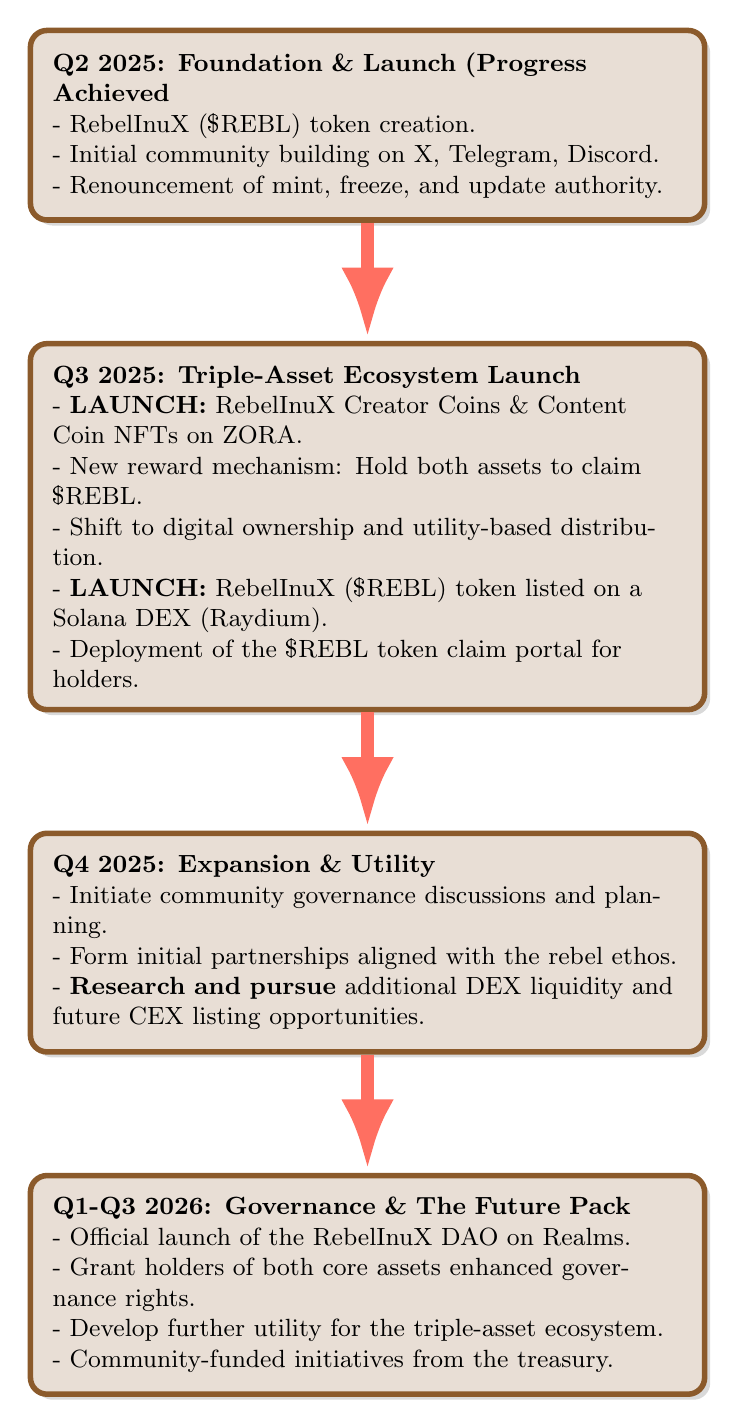
\begin{tikzpicture}[
  node distance=1.5cm and 0cm,
  every node/.style={
    rectangle,
    draw=primaryColor, 
    fill=primaryColor!20, 
    rounded corners=6pt,
    line width=2pt,
    drop shadow={shadow xshift=2pt, shadow yshift=-2pt, opacity=0.3},
    align=left,
    text width=8cm,
    inner sep=8pt,
    font=\small
  },
  arrow/.style={
    -Latex,
    thick,
    draw=accentColor,
    shorten >=1pt,
    line width=5pt
  }
]
 % Define nodes - UPDATED
  \node (Q2) {\textbf{Q2 2025: Foundation \& Launch (Progress Achieved}
    \\- RebelInuX (\$REBL) token creation.
    \\- Initial community building on X, Telegram, Discord.
    \\- Renouncement of mint, freeze, and update authority.};
  \node (Q3) [below=of Q2] {\textbf{Q3 2025: Triple-Asset Ecosystem Launch}
    \\- \textbf{LAUNCH:} RebelInuX Creator Coins \& Content Coin NFTs on ZORA.
    \\- New reward mechanism: Hold both assets to claim \$REBL.
    \\- Shift to digital ownership and utility-based distribution.
    \\- \textbf{LAUNCH:} RebelInuX (\$REBL) token listed on a Solana DEX (Raydium).
    \\- Deployment of the \$REBL token claim portal for holders.};
  \node (Q4) [below=of Q3] {\textbf{Q4 2025: Expansion \& Utility}
    \\- Initiate community governance discussions and planning.
    \\- Form initial partnerships aligned with the rebel ethos.
    \\- \textbf{Research and pursue} additional DEX liquidity and future CEX listing opportunities.};
  \node (Q1) [below=of Q4] {\textbf{Q1-Q3 2026: Governance \& The Future Pack}
    \\- Official launch of the RebelInuX DAO on Realms.
    \\- Grant holders of both core assets enhanced governance rights.
    \\- Develop further utility for the triple-asset ecosystem.
    \\- Community-funded initiatives from the treasury.};

  % Connect nodes with arrows
  \draw[arrow] (Q2.south) -- (Q3.north);
  \draw[arrow] (Q3.south) -- (Q4.north);
  \draw[arrow] (Q4.south) -- (Q1.north);
\end{tikzpicture}
\end{center}

% Add this disclaimer right after the roadmap graphic
\begin{center}
\fbox{
\begin{minipage}{0.8\textwidth}
\small
\centering
\textit{\textbf{Note on Timelines:} This roadmap outlines our strategic goals and estimated timeframes. Development is complex and unpredictable. These dates are forecasts, not promises, and may shift based on technical challenges, community feedback, and market conditions. Our commitment is to build a quality ecosystem, not to rush to meet deadlines.}
\end{minipage}
}
\end{center}
\vspace{0.5em}
\begin{center}
\textit{\underline{The Evolving Path of the Rebellion}}
\end{center}
\vspace{1em}

\vspace{1em}

% About the Founder with styling
% About the Founder with styling
\section[
\texorpdfstring{\color{primaryColor}About the Founder}{About the Founder}
]{\color{primaryColor}\textbf{About the Founder}}

\begin{tcolorbox}[colback=headerColor!10!white, colframe=headerColor, boxrule=0.8mm, width=\textwidth]
\textbf{Clément Landormy} — A dedicated expert in cryptoassets and blockchain technology with over three years of specialized experience gained through his PhD in economics. His expertise encompasses cryptoasset valuation, econometrics, and market analysis.

Clément has conducted extensive empirical research using on-chain data from Binance, Coinbase, and CoinMetrics, focusing on market risks, asset pricing, and financial forecasting. He is proficient in quantitative analysis, financial modeling, programming, and data visualization.

His mission is to develop transparent, innovative, and community-driven blockchain projects that advance the industry and foster trust within the ecosystem.
\end{tcolorbox}

\vspace{1em}

\section[
\texorpdfstring{\color{primaryColor}Meet Our Inspiration: RebelInuX’s Model}{Meet Our Inspiration: RebelInuX’s Model}
]{\color{primaryColor}\textbf{Meet Our Inspiration: RebelInuX’s Model}}
\begin{tcolorbox}[colback=headerColor!10!white, colframe=headerColor, boxrule=0.8mm, width=\textwidth, arc=6mm, left=8mm, right=8mm, top=6mm, bottom=6mm]

\textbf{RebelInuX is more than just a meme coin — it’s a reflection of the loyalty, playfulness, resilience, and strong character embodied by our beloved dog, Idilys.}

\subsection*{About Idilys}

Idilys is a Shiba Inu known for her unwavering loyalty, sharp intelligence, courage, and strong personality. She’s a true rebel at heart — she doesn’t listen much to orders and hates being on a leash. Despite her independence, she’s loving and fiercely loyal. She embodies the spirit of rebellion, community, and perseverance, serving as the perfect symbol of strength and freedom.

\subsection*{Why Idilys?}

Our dog serves as the mascot and inspiration for RebelInuX because:

\begin{itemize}
  \item \textbf{Loyalty}: Like our community, Idilys is fiercely loyal and dedicated.
  \item \textbf{Resilience}: Always bouncing back, just like our token aims to grow and adapt.
  \item \textbf{Independence}: She’s strong-willed and refuses to be controlled — a true reflection of rebellion.
  \item \textbf{Playfulness}: Bringing joy and fun, which is at the heart of our meme culture.
\end{itemize}

\end{tcolorbox}

\section[
\texorpdfstring{\color{primaryColor}Join the Rebel Pack and Unleash the Rebellion}{Join the Rebel Pack and Unleash the Rebellion}
]{\color{primaryColor}\textbf{Join the Rebel Pack and Unleash the Rebellion}}

We believe in challenging the status quo—fighting injustices in the crypto sphere and beyond. As a community, we stand united in pushing boundaries, standing up for what's right, and making a difference. We are building more than just a token; we are building a movement powered by a **triple-asset ecosystem** of digital ownership and value.

\textit{Together, we are more than just a meme — we are a rebellion that fights for change.}

\vspace{0.5em}

\begin{center}
  \includegraphics[width=0.4\textwidth]{RebelInuX — Unleash the roar - Imgur.jpg}
  \\ % Line break for the caption
  \small\textit{Figure 2: "RebelInuX — Unleash the roar" – One of the RebelInuX Content Coin NFTs. Explore the collection on ZORA.}
\end{center}

\vspace{0.5em}

Become part of the wildest crypto movement. Connect with the community, explore our digital assets, and join the conversation on our official channels:

\begin{itemize}
  \item \textbf{Explore the Core Assets:} \href{https://zora.co/@rebelinux}{ZORA Collection (Creator Coins \& Content Coin NFTs)}
  \item \textbf{Follow the News:} \href{https://x.com/RebelInuX}{Twitter}
  \item \textbf{Join the Chat:} \href{https://t.me/+bNrP-ozjM501YWVk}{Telegram}
  \item \textbf{Connect with the Community:} \href{https://discord.gg/3gBzGY6j}{Discord}
\end{itemize}

Join us and help build a vibrant, rebellious ecosystem that stands strong together!

\section[
\texorpdfstring{\color{primaryColor}Token Creation and Verification}{Token Creation and Verification}
]{\color{primaryColor}\textbf{Token Creation and Verification}}

\noindent
The \textbf{RebelInuX (\$REBL)} token was officially created on \textbf{18 June 2025} at \textbf{20:38 UTC} using \href{https://oriontools.io}{OrionTools.io}, a trusted platform for deploying Solana-based tokens.

\vspace{0.5em}
\noindent
\textbf{Solana Token Address:}
\begin{center}
    \href{https://solscan.io/token/BfVVGU2an66FVL6qCrx8gJDdgw6EwzmjG672YYD7REmM}{\ttfamily BfVVGU2an66FVL6qCrx8gJDdgw6EwzmjG672YYD7REmM}
\end{center}

% --- VERIFICATION SUBSECTION - REPLACES THE REDUNDANT PARAGRAPH ---
\subsection*{On-Chain Verification}
\begin{itemize}
    \item \textbf{\$REBL Token Contract:} The permanent renouncement of the Mint, Freeze, and Update Authorities can be verified on any Solana block explorer (e.g., \href{https://solscan.io/token/BfVVGU2an66FVL6qCrx8gJDdgw6EwzmjG672YYD7REmM}{Solscan}) using the address above.
    \item \textbf{ZORA NFT Collections:} The Creator Coin and Content Coin NFT collections can be viewed and verified on the ZORA platform: \href{https://zora.co/@rebelinux}{https://zora.co/@rebelinux}. The Creator Coin contract address on Base is: \href{https://basescan.org/token/0xf95beef6439ec38fa757238cdec8417abda536bd}{\texttt{0xf95beef...a536bd}}
\end{itemize}

\bigskip
\noindent
This documentation ensures that the creation process and security claims are transparent and verifiable by all community members and stakeholders.

\begin{tcolorbox}[colback=red!5!white, colframe=red!75!black, title=\textbf{\large WARNING: Important Market Considerations \& Risks}, fonttitle=\bfseries, arc=3mm]



\subsection*{Volatility \& Market Manipulation}
Participants in the RebelInuX ecosystem should be aware of the highly volatile and speculative nature of cryptoasset markets. Upon the launch of our initial liquidity pool, which will start with a controlled depth, it is common for automated bots and large-scale traders ("whales") to engage in market manipulation strategies. This can include:

\begin{itemize}
    \item \textbf{Extreme Price Volatility:} Rapid and significant price increases ("pumps") and decreases ("dumps").
    \item \textbf{"Sniping" and Front-running:} Bots may execute transactions before others, gaining an unfair advantage.
\end{itemize}

\noindent
\textbf{This activity is an external feature of the trading environment and is not initiated by, nor within the control of, the RebelInuX team.} Our foundational mitigations against malicious activity are:

\begin{itemize}
    \item The permanent renouncement of mint, freeze, and update authorities.
    \item The locking of \textbf{90\% of the initial liquidity pool (LP) tokens}. The remaining portion is held in a secure multisig wallet for future community-approved initiatives, such as additional trading pairs.
\end{itemize}

\noindent
Investors should exercise extreme caution, conduct their own research (DYOR), and never invest more than they are willing to lose. The RebelInuX project is focused on long-term utility and growth, not short-term price action.
\end{tcolorbox}
% Legal Disclaimer
\begin{tcolorbox}[colback=backgroundColor!10!white, colframe=headerColor, boxrule=0.8mm, title=Legal Disclaimer, fonttitle=\bfseries]
RebelInuX is a community-driven memecoin project designed for entertainment and community engagement. This token is not a security, investment, or financial product and should not be viewed as such. It confers no ownership, equity, or financial rights. Its value is derived solely from community participation and speculative demand.
\medskip
\noindent
\fbox{\begin{minipage}{\textwidth}
\centering
\textbf{\large AVERTISSEMENT POUR LES RÉSIDENTS FRANÇAIS} \\
    \textbf{Interdit aux résidents français.} \\En raison des restrictions réglementaires de l'AMF (Autorité des Marchés Financiers), les résidents et citoyens français sont expressément interdits d'acheter, de détenir ou d'échanger le jeton RebelInuX.
\end{minipage}}

\medskip
\noindent
Cryptocurrency investments carry risks, including potential loss of principal. Please conduct your own research and consult with a professional before participating. RebelInuX does not guarantee any financial returns or profits and is not responsible for any damages caused by participation in this project.
\end{tcolorbox}


\vspace{1em}

\begin{center}
\small \textcopyright\, 2025 \\
RebelInuX \quad | \quad \textit{Created by Clément Landormy} \\
All rights reserved.
\end{center}

\end{document}